%
\section{Moving converter to OPA}

Make degrader of CH2 , 24mm thick) and move the converter to OPA .

{\red TODO: need a figure with the geometry drawing}

\begin{itemize}
\item
  Generate 10M events
\item 
  The simulated range of cos(theta) is [0,0.45] - dataset family rpc07b0
\end{itemize}

\begin{figure}[H]
  \begin{tikzpicture}
    \node[anchor=south west,inner sep=0] at (0,0.) {
      % \node[shift={(0 cm,0.cm)},inner sep=0,rotate={90}] at (0,0) {}
      \makebox[\textwidth][c] {
        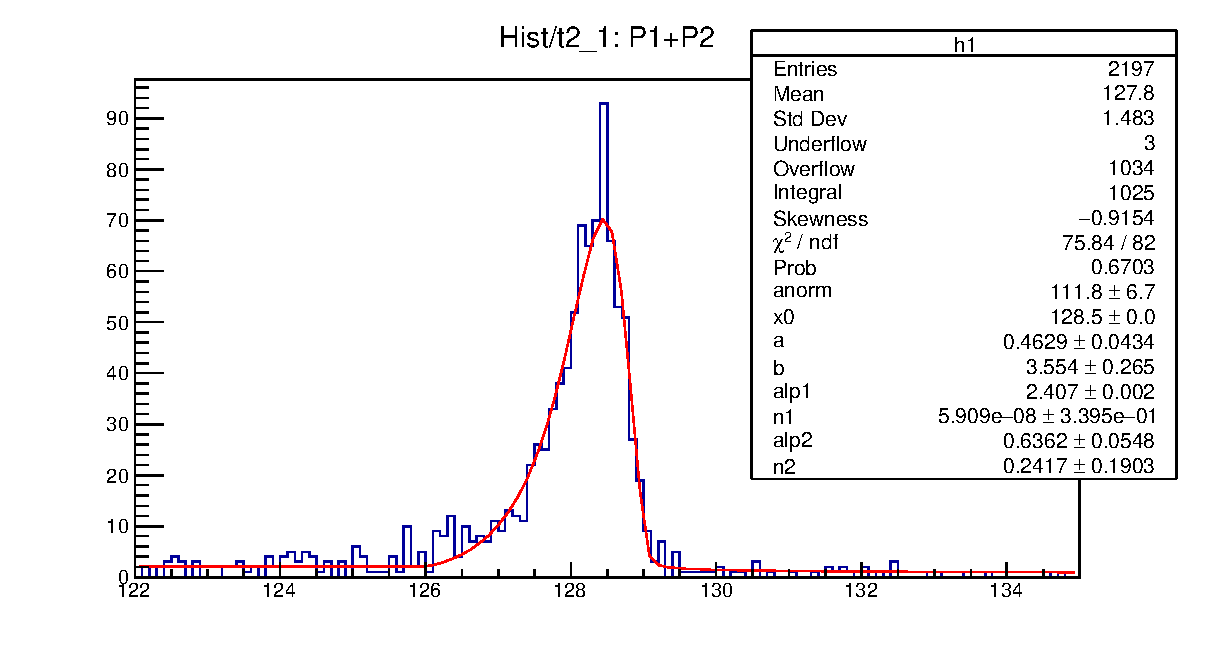
\includegraphics[width=0.95\textwidth]{pdf/pipenu_rpc07b0s51r0100_drpc_ana_t2_1_smom_1_fit}
      }
    };
    % \node [text width=8cm, scale=1.0] at (14.5,0.5) {$\mu_B$, expected background mean};
    % \node [text width=8cm, scale=1.0, rotate={90}] at (1.5,7.5) { $S_{D}$, ``discovery'' signal strength  };
  \end{tikzpicture}
  \caption{
    \label{figure:t2_1_smom_0}
    Sum of the two reconstructed track momenta and its fi.t 2cm wide converter in OPA
  }
  \label{figure:event_display}
\end{figure}

%%%%%%%%%%%%%%%%%%%%%%%%%%%%%%%%%%%%%%%%%%%%%%%%%%%%%%%%%%%%%%%%%%%%%%%%%%%%%%
%%%%%%%%%%%%%%%%%%%%%%%%%%%%%%%%%%%%%%%%%%%%%%%%%%%%%%%%%%%%%%%%%%%%%%%%%%%%%%
\newpage
\subsection{TSdA : impact on the CE acceptance}

Figure~\ref{figure:ce_momentum_tsda} compares acceptances for the reconstructed CE tracks
got default geometry and geometry w/o the TSdA.
\begin{itemize}
\item 
  CE on Al for this comparison have been generated with the radiative corrections
  taken into account in the LL approximation.
\item 
  A model of perfect detector has been used - no misalignments, no miscalibrations.
\item
  2.5M events simulated per configuration.
\end{itemize}


\begin{figure}[H]
  \begin{tikzpicture}
    \node[anchor=south west,inner sep=0] at (0,0.) {
      % \node[shift={(0 cm,0.cm)},inner sep=0,rotate={90}] at (0,0) {}
      \makebox[\textwidth][c] {
        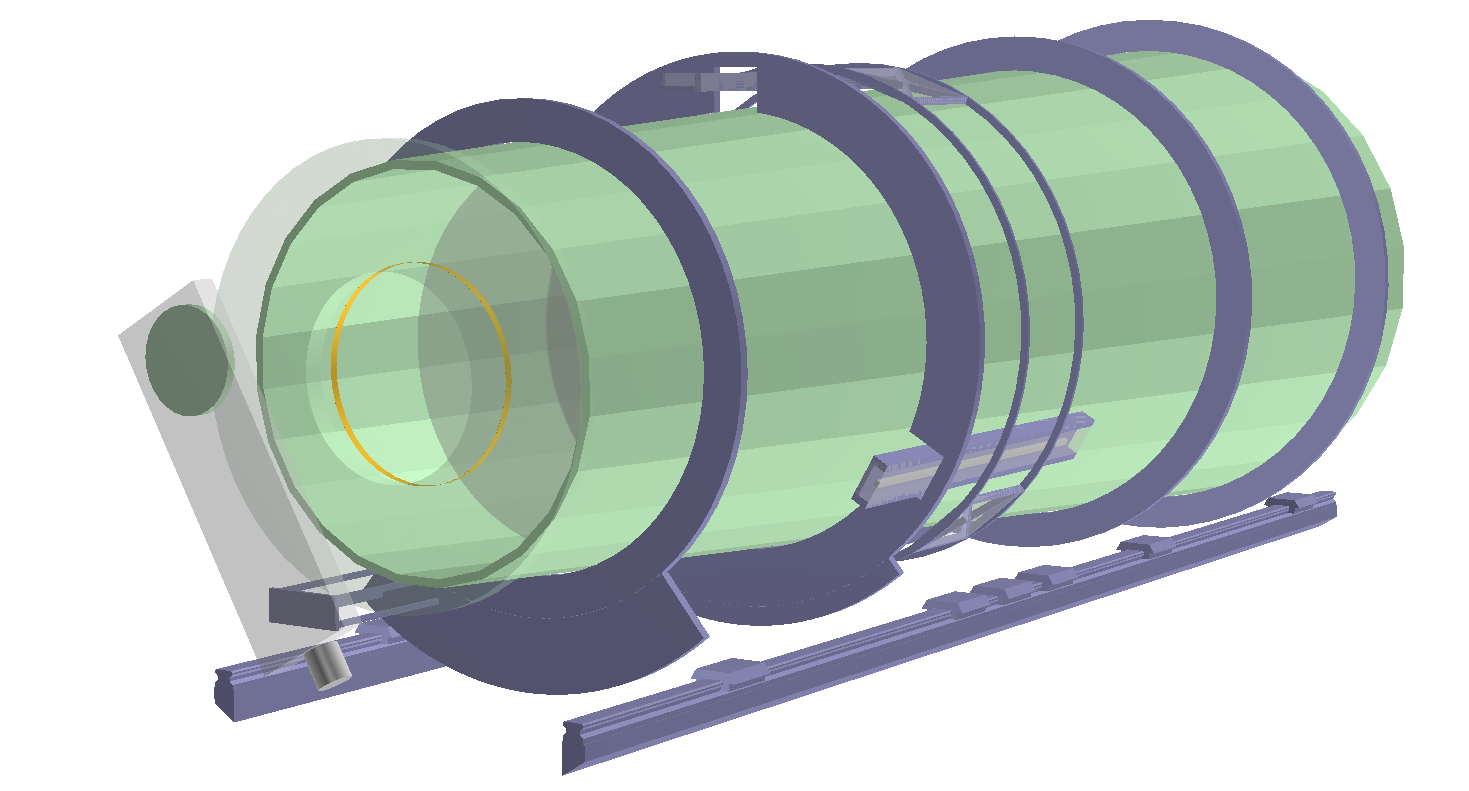
\includegraphics[width=0.90\textwidth]{png/pipenu_cele3b0_geom_degrader}
      }
    };
    % \node [text width=8cm, scale=1.0] at (14.5,0.5) {$\mu_B$, expected background mean};
    % \node [text width=8cm, scale=1.0, rotate={90}] at (1.5,7.5) { $S_{D}$, ``discovery'' signal strength  };
  \end{tikzpicture}
  \caption{
    \label{figure:degrader_v4}
    degrader v4: converter ring supported by OPA
  }
\end{figure}


Plotted: all reconstructed tracks, no selections

Comparison of the distributions tells that the presence of the TSdA doesn't impact the CE acceptance.

\begin{figure}[H]
  \begin{tikzpicture}
    \node[anchor=south west,inner sep=0] at (0,0.) {
      % \node[shift={(0 cm,0.cm)},inner sep=0,rotate={90}] at (0,0) {}
      % \makebox[\textwidth][c] {
        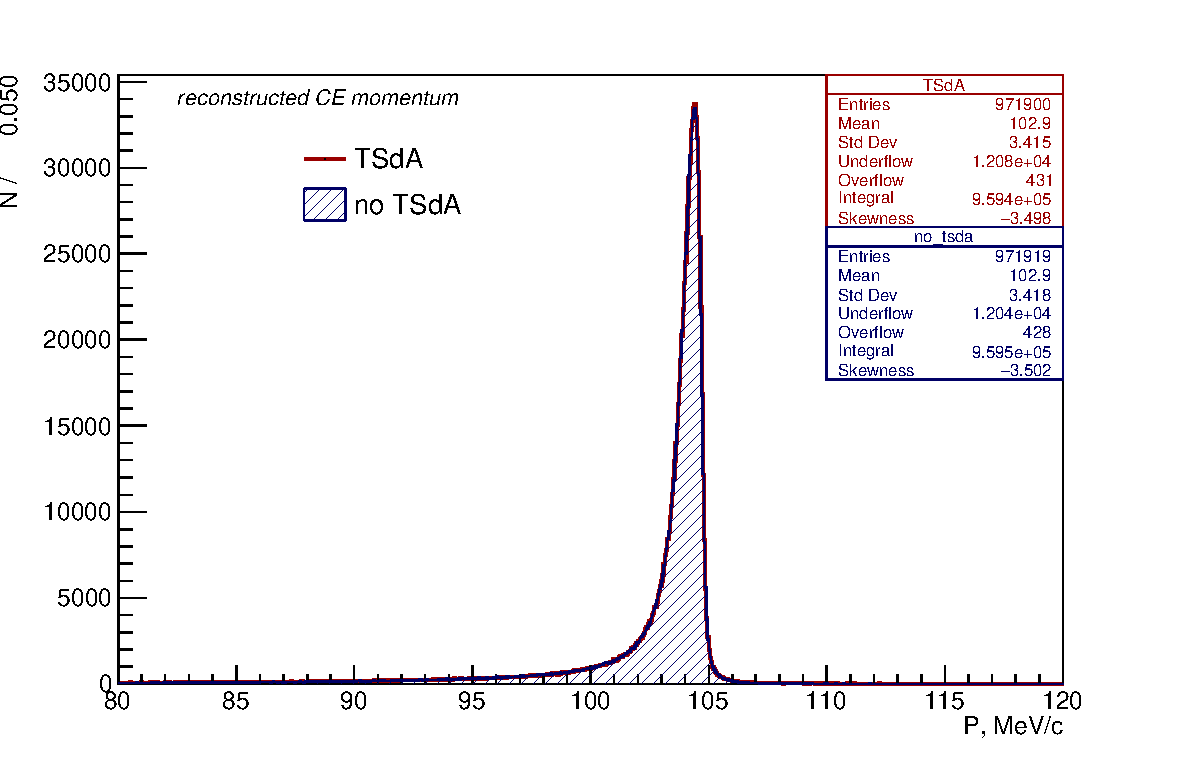
\includegraphics[width=0.54\textwidth]{pdf/figure_00061}
      % }
    };
    \node[anchor=south west,inner sep=0] at (9.8,0.) {
      % \node[shift={(0 cm,0.cm)},inner sep=0,rotate={90}] at (0,0) {}
      % \makebox[\textwidth][c] {
        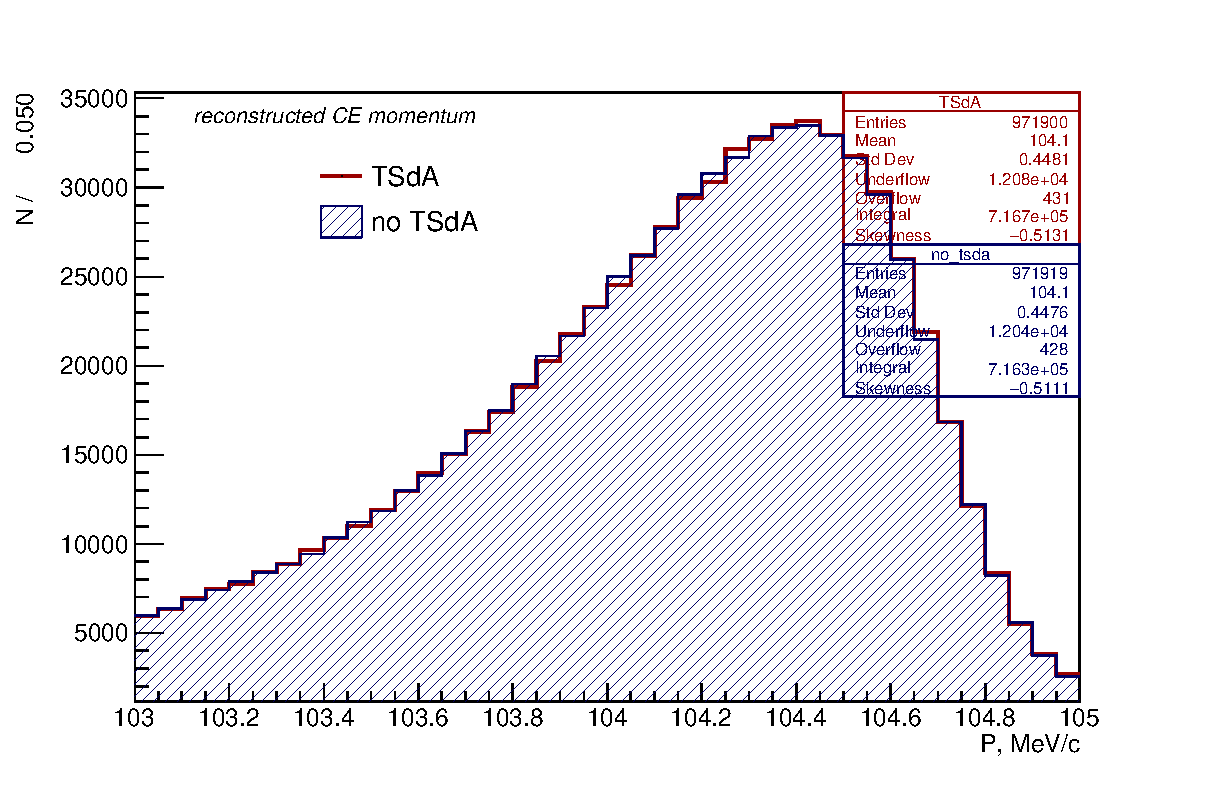
\includegraphics[width=0.54\textwidth]{pdf/figure_00062}
      % }
    };
    % \node [text width=8cm, scale=1.0] at (14.5,0.5) {$\mu_B$, expected background mean};
    % \node [text width=8cm, scale=1.0, rotate={90}] at (1.5,7.5) { $S_{D}$, ``discovery'' signal strength  };
  \end{tikzpicture}
  \caption{
    \label{figure:ce_acceptance}
    CE momentum distribution for two geometries, with an without the TSdA
  }
  \label{figure:ce_momentum_tsda}
\end{figure}
%%% Local Variables:
%%% mode: latex
%%% TeX-master: t
%%% End:
